\chapter{Implementation: The Mapping}
\label{chapter:impl_mapping}

In this chapter we will describe the implementation of the model transformations from BPMN to BPEL and JIAC.

The methodology for both transformations is very similar. The mappings have been realized using the EMT framework, which has been introduced in section \ref{sec:emt}. However, the EMT framework has been used without its visual editor, which still seemed to be too unstable. Instead the framework has been optimized for manual use, meaning that with no big effort the rules can be directly implemented in Java instead of using the EMT compiler.

After giving a overview of the project and plugin structure we will introduce the Transformation Base, that is, the modified EMT framework, and the codomain models. After that we will explain in detail the stages of the mapping, from the normalization to the clean up, including the several rules designed to transform the rather unstructured BPMN graphs to structured BPEL and JIAC models. Finally we will discuss the remaining open issues.



\section{Project Structure}

Like the editor feature, the mapping features are spread across several interdependent plugins, as shown in figure \ref{fig:impl_struc_mapping}. Again we will give a short description of the plugins. Note that every export feature may provide its own plugins which are not required to follow this structure used for the export features in this diploma thesis.

\begin{figure}[htp]
	\centering
	\includegraphics[width=.75\textwidth]{figures/impl/struc_mapping.png}
	\caption[Mapping-Plugin Interdependencies]{Mapping-Plugin Interdependencies. Components at the top of the figure require those at the bottom (transitively). Different colors mark a possible composition in Features.}
	\label{fig:impl_struc_mapping}
\end{figure}

\begin{itemize}
	\item \texttt{TransformationBase} This plugin is holding the classes needed for the rule based transformation. These are the slightly modified and optimized classes generated by the EMT framework. This plugin can be used for any EMF model transformation, independently of the source and target language.
	\item \texttt{BpmnExport.refmodel} The reference model connecting the source model with the target model. The reference model is independent of the target language and can be used for the transformation to both BPEL and JIAC.
	\item \texttt{BpmnExport.rules} This plugin is holding those parts of the rules that are independent of the target language. It provides the normalization rules, which operate on the source model only, as well as the wrapper classes for the rules of the structure mapping, which provide the patterns for the pattern matching and are independent of the target language, too.
	\item \texttt{BPEL} This plugin is holding the BPEL metamodel.
	% \item \texttt{BPEL (.edit,.editor)} These plugins are holding the BPEL metamodel and a standard EMF editor for it.
	\item \texttt{BPEL.edit, BPEL.editor} These plugins are required for providing a standard EMF editor for the BPEL models. They are not needed for the export functionality but may be useful for easier validation and editing of the resulting model.
	\item \texttt{Bpmn2Bpel.export, Bpmn2Jiac.export} These plugins are holding the logic needed for the export to BPEL and JIAC, including the export wizard, a visitor and the remaining rules. The JIAC export plugin also contains the libraries holding the JIAC IV metamodel and code generation routines, which are realized using JAXB.
\end{itemize}

Note that neither the \texttt{TransformationBase} nor the \texttt{.export} plugin do require any of the EMT plugins. All classes needed for the application of the rules are contained in the TransformationBase plugin and no other plugins than those already required for the editor are needed.



\section{The Transformation Base}
\label{sec:impl_emt}

The TransformationBase plugin is based on the EMT framework introduced in section \ref{sec:emt}.
The plugin consists of only 11 classes. The \verb|Transformation| class is aggregating a set of rules and tries to execute them as long as possible. The \verb|AbstractRule| class is providing the methods needed for the rules while the \verb|AbstractWrapper| class is the superclass for ``wrappers'', which define the rule's left hand side (LHS) and negative application conditions (NACs) and are used for the pattern matching, which is done by the \verb|Matchfinder| class. For each object in a rule's LHS a \verb|Variable| is defined. A number of \verb|Queries| are assigned to the Variables which have to be fulfilled in the course of the pattern matching algorithm so that the rule can be applied.

These classes were first generated by the EMT compiler and have then been optimized with respect to easier maintainability and performance. Some minor bugs have been fixed and the backtracking algorithm has been optimized, too, making it more efficient. A number of sub routines have been written, simplifying the creation of Variables and Queries.

The generated rule implementations had to use EMF's reflective API. For creating a instance of a EClass (that is, a EObject) the class had to be searched for by its name in each EPackage that has been assigned to the transformation model. Obviously this is not very performant, hard to maintain and error prone -- what if there are two EClasses with the same name? This is not needed anymore when writing the rules by hand, so the resulting rule classes are relatively slim while still using the benefits of the transformation framework, for instance the fully implemented pattern matching algorithms.

Another benefit of not using the graphical rule editor is not being bound to its restrictions. A ``classical'' rule has a Left Hand Side (LHS, the pattern), some Negative Application Conditions (NAC), conditions and \emph{one} Right Hand Side (RHS, the result). This is not very advantageous in the case of BPMN, since most elements of BPMN have several sub types, which have great influence on the mapping. The differences between the several sub types can not be expressed in a rule's single RHS, so for each subtype a new rule would need to be created. Let alone all the possibilities of containing elements for each of these types! Using the classical LHS-RHS approach would have resulted in literally \emph{hundreds} of rules.

Thus the most important change is the introduction of the \verb|Rule.apply()| method, replacing the existing methods for building the rule's RHS. The old methods were subdivided into creating, changing and removing objects in the RHS. Having only one single method for creating, changing and deleting objects in the course of the rule's execution, the readability and maintainability of the rule classes is increased a lot and new elements, such as conditionals and loops, can be introduced.



\section{The Codomain Models}

This section will outline the metamodels for the target languages.% needed for the mapping.

\paragraph*{BPEL and WSDL}

The EMF Ecore models for the Business Process Execution Language (BPEL) and Web Service Definition Language (WSDL) were created from the BPEL XML Schema Definition (XSD) \cite[Appendix D]{spec_bpel}. Thus, the model's XML code is equal to the original BPEL XML code and no transformation from one to the other is needed.

\paragraph*{JIAC}

The JIAC domain model was taken without modifications from the existing JIAC IV projects. Along with the model all the code generation routines could be reused.

Unfortunately the existing JIAC metamodel is implemented in JAXB\footnote{\url{http://java.sun.com/webservices/jaxb/}}. This has the consequence that JIAC model elements can not be used in the EMT pattern matching. They can be created in the course of the rule's application, though. This has no impact on the actual mapping, since in these stages only the source model and the reference model are needed for the pattern matching. But with this restriction it is not possible to write clean up / beautifier rules for JIAC using the EMT framework.

The next version of JIAC, JIAC TNG, will be based on EMF. As soon as JIAC TNG is available the transformation should be converted to JIAC TNG, including a beautifier.

\paragraph*{The Reference Model}

For the rule based transformation a minimal reference model has been developed (see figure \ref{fig:model_ref}). This model's purpose is to hold the source and target models together. The Mapping Root is holding references to the BPMN root element, namely the Business Process Diagram, and the target language's top-level structures. Further it holds a list of References, which subdivide in Activity References and Sequence References. These are needed to connect each element of the source model with its representation in the target model. Additionally they mark an element as being processed simply by referencing it. This can be used as a pattern in a Negative Application Condition (NAC) in the transformation rules to prevent the rule from being executed twice for the same element. While Activity References permanently connect each Activity of the source model with its counterpart in the target model, Sequence References, which are used to connect sequences to be created in the target model with the first and the last node belonging to that sequence in the source model, are reduces in the course of the transformation.

\begin{figure}[htp]
	\centering
	\includegraphics[width=.6\textwidth]{figures/impl/models/model_ref.png}
	\caption[The Reference Model]{The Reference Model. The MappingRoot element is containing both the source and target model.}
	\label{fig:model_ref}
\end{figure}

The reference model is independent of the source and target model. While the Reference types are tailored to fit workflow models all the references to the source and target model elements have the type \verb|Object| and thus can be used with any metamodel.



\section{Stages of the Mapping}

The transformation has been subdivided into several stages which are finished one after another. Some of these stages are identical for each mapping, independent of the target language. Others are similar in their structure but have to be implemented individually for each target language.

\begin{enumerate}
	\item \textbf{Normalization}: Puts the model in a uniform form to facilitate the later stages.
	\item \textbf{Element Mapping}: Transformation of the several activities to a unsorted collection of concurrent sequences.
	\item \textbf{Structure Mapping}: Mapping of control flow, combining the previously created sequences in larger structures.
	\item \textbf{Cleaning Up}: Cleaning up the resulting workflow.
\end{enumerate}

The central component in the transformation is the \emph{Visitor}. It extends the reference model's MappingRoot class and thus holds the References connecting the source and target models. At first it calls the pre transformation, that is the \emph{Normalization Stage}, then it starts its top-down traversion, the \emph{Element Mapping}. After that the post transformation is called, which consists of the \emph{Structure Mapping} and the \emph{Clean Up}. Finally the results are saved in the directory that has been specified by the user. In the following sections we will explain the several stages in detail.


\subsection{Normalization}

This is the first stage of the transformation and a internal transformation of the source model. Thus this stage is completely independent of the target language. This stage is intended to put the model in a uniform structure to facilitate the following stages of the transformation. The model will not be saved after the transformation, thus the changes done here won't affect the model file.
%This stage could also be used to validate the model and to check if there is any structure that can not be mapped.\footnote{Although the editor is providing model validation there might be models that are valid according to the BPMN specification and still can not be mapped due to insufficiencies in the target language or the definition of mapping.}.

Each of the normalization rules presented here are very short and concise. Often the LHS consists of only one or two elements. Thus it does pay of highly if the number and complexity of rules needed for the Structure Mapping can be reduced by introducing these normalization rules. In the following paragraphs we will introduce some of the normalization rules and give a high level view on the diagram before and after the application of the rule.

\subsubsection*{Split Gateway Rule}
With this rule Gateways with both multiple incoming and outgoing Sequence Flows are split in two Gateways, one with multiple incoming, the other with multiple outgoing Sequence Flows (see figure \ref{fig:split_gateway}). This rule is necessary for facilitating the Block Rule, which will be covered later on in this chapter. After the application of this rule each Gateway is either a forking Gateway or a merging Gateway.

\begin{figure}[htp]
	\centering
	\includegraphics[width=.6\textwidth]{figures/impl/rules/split_gateway.png}
	\caption[Split Gateway Rule]{The Split Gateway Rule.}
	\label{fig:split_gateway}
\end{figure}

\subsubsection*{Insert Gateway Rule}
With this rule an Activity with multiple incoming and/or outgoing Sequence Flows is split up in the Activity alongside with one or two Gateways (see figure \ref{fig:insert_gateway}). This rule is necessary to facilitate the Sequence Rule and the Block Rule. After the application of this rule each Activity will have at most one incoming and outgoing Sequence Flow.

\begin{figure}[htp]
	\centering
	\includegraphics[width=.6\textwidth]{figures/impl/rules/insert_gateway.png}
	\caption[Insert Gateway Rule]{The Insert Gateway Rule for the case of multiple outgoing Sequence Flows.}
	\label{fig:insert_gateway}
\end{figure}

\subsubsection*{Insert Empty Rule}
With this rule two Gateways that are directly connected by a Sequence Flow are separated by an Activity with task type \verb|None| (see figure \ref{fig:insert_empty}). The Activity will be mapped to a no-op activity in the target language and can eventually be removed in the \emph{Clean Up} layer. This rule is necessary to facilitate the Block Rule and Loop Rule. After the application of this rule there will be no directly connected Gateways anymore, meaning that there are not empty sequences between Gateways and that every sequence spanning from one Gateway to another is beginning and ending with a Activity with only one incoming and outgoing Sequence Flow.

\begin{figure}[htp]
	\centering
	\includegraphics[width=.6\textwidth]{figures/impl/rules/insert_empty.png}
	\caption[Insert Empty Rule]{The Insert Empty Rule.}
	\label{fig:insert_empty}
\end{figure}

\subsubsection*{Example}
Figure \ref{fig:normalization_example} is showing a short example of how the Normalization rules help to change a loop structure drawn in a very short and easily understandable way to a more extensive representation with exactly the same semantics that can be mapped by the Loop Rule, being introduced in the \emph{Structure Mapping}.

\begin{figure}[htp]
	\centering
	\includegraphics[width=.75\textwidth]{figures/impl/rules/normalization_example.png}
	\caption[Normalization example]{Application of two normalization rules to alter a loop structure so it can be mapped in the structure mapping.}
	\label{fig:normalization_example}
\end{figure}

\subsubsection*{Processing of Unstructured Workflows}
Another part of the normalization mapping would be the structuring of unstructured workflows, as introduced in section \ref{sec:mda_mapUSWF}. This part of the mapping has not yet been implemented in this work, thus only workflows that are already in a structured form -- apart from the minor defects stated above -- can be mapped. Some more research will be needed before this part of the mapping can be completed and a number of additional rules will be necessary to cover each possibility of unstructured workflows.


\subsection{Element Mapping}

The second stage of the mapping, the \emph{Element Mapping}, is the only stage that is not rule based. Instead the mapping of the several BPMN elements to their correspondents in BPEL and JIAC has been implemented using a visitor-like top-down traversion of the source model. A rule based transformation would have been possible, too, but not necessary in this case, and a set of rules would be much harder to debug and to maintain. Further, the top-down traversion is faster that the pattern matching required for a rule based transformation.

With this stage of the mapping two new models will be build alongside the source model: The reference model and the target model. While in some other transformations the source model often is annotated and reduced, the source model will stay intact in our case. Instead the reference model is used to connect it with the target model to be created. This has the advantage that the whole source model is still available for checks and rule patterns later on.

For each element of the source model -- that is, mainly the Pools and Flow Objects -- a corresponding element of the target language will be created and connected to the source element with Reference objects. However, these elements are only loosely gathered in a parallel structure. The right execution order, alternative paths and concurrency will be added later, in the Structure Mapping.

The visitor is starting at the root element, the Business Process Diagram. One program module, that is, a BPEL process or a JADL planelement, is created for each Pool in the diagram. For the Pool as a whole a parallel structure in created, the Pool's elements are traversed and the corresponding elements of the target language are created. If no mapping is defined for some element than a no-operation element is created with a short description, for instance the original element's name. In BPEL this will be an \verb|empty| activity, in JIAC a \verb|logwarn|. For each mapping an \emph{Activity Reference} is created and referenced by the Mapping Root. These objects are holding references to the mapped element and its counterpart in the target language and are needed for some of the transformations in the Structure Mapping.

In BPMN each Flow Object can have Assignments, which do not have a graphical representation in the diagram. These Assignments are mapped to assignments in the target language, e.g. an \verb|assign| in BPEL or a \verb|bind| in JIAC. These assignments, together with the Flow Object's mapping, are wrapped in a sequence element. For this sequence a \emph{Sequence Reference} is created, which is needed for the next stage, the Structure Mapping, and is registered at the Mapping Root object\footnote{which actually is the Visitor itself}.

Finally the sequence is inserted into the parallel structure together with the sequences that have been created for the other Flow Objects in the same (Sub-) Process. Later, in the Structure Mapping, these sequences will be combined to larger sequences, decision structures and loops. Sequences, that can not be combined, remain concurrent in the parallel structure. Figure \ref{fig:elemMapping} should illustrate the concept.

\begin{figure}[ht]
	\centering
	\includegraphics[width=.5\textwidth]{figures/impl/elemMapping.png}
	\caption[Use of Sequences in Element Mapping]{Using sequences to wrap mappings of FlowObjects and Assignments in the Element Mapping. Yellow: Source Model, Green: Reference Model, Red: Target Model.}
	\label{fig:elemMapping}
\end{figure}


\subsection{Structure Mapping}

A great challenge consisted in mapping the BPMN diagram graphs to the structured executable languages. While BPMN diagrams are directed graphs, BPEL and JADL are block oriented. This means that each loop or block structure has to have exactly one entry and one exit point. It is not possible to ``break out'' of the block or to alternate between two concurring blocks.

Mapping a directed graph to an equivalent block structure consists of two steps: Firstly one has to alter the diagram in an endogenous transformation so it will be in a block structure, then the exogenous transformation to the target language can begin.

The first step should be done in the Normalization stage of the mapping, so that new elements can be regarded in the Element Mapping. So everything that's left at this point is to identify graph structures that can be mapped to block structures.

% drei haupt-regeln, mit denen sich schon so einiges machen lässt
As written earlier in section \ref{sec:mda_mapUSWF} a structured workflow model basically consists of only three elements: Sequences, choice/parallel blocks and loops. In BPMN there are various possibilities of realizing these structures \cite{patterns1,patterns2}. Still three rules are enough to cover the biggest part of the Structure Mapping.

\begin{enumerate}
	\item \textbf{Sequence Rule}: Those sequences in the target model corresponding to Flow Objects connected with a Sequence Flow are combined to larger sequences.
	\item \textbf{Block Rule}: Blocks in the BPMN diagram are identified and a corresponding block structure is created in the target model.
	\item \textbf{Loop Rule}: Loops are identified and a loop structure is created. The until- and the while-parts of the loop are put in the structure.
\end{enumerate}

% anmerkung: weitere, ähnliche regeln für spezialfälle davon, wie loops, einelementige sequenzen, etc.
Note that these three rules are still not enough to do the whole Structure Mapping. Some more rules are needed for special cases like open blocks, that is, blocks that are defined by only the forking or the merging Gateway. These blocks are essential for defining workflows with multiple Start or End Events. Further BPMN's exception handling does require some additional rules. All these rules are basically very similar to the three rules presented here and will not be explained in detail.

The figures \ref{fig:seqRule}, \ref{fig:blockRule} and \ref{fig:loopRule} will roughly illustrate the three main rules. The yellow nodes are elements of the source model, BPMN. The red nodes are elements of the target model, BPEL or JIAC. The green nodes are elements of the reference model, connecting the source and target model. The area within the dotted rounded rectangle is the pattern that has to be matched in the source model.

\subsubsection*{Sequence Rule}
In this rule, shown in figure \ref{fig:seqRule}, sequences of sequences are merged to larger sequences. It is necessary that in the Element Mapping each resulting element of the target language has been initially wrapped in a sequence and referenced by a Sequence Reference. If this has been done each of these elements will be both \verb|first| and \verb|last| and the Flow Object's incoming and outgoing Sequence Flows will be the \verb|incoming| and \verb|outgoing| of that Sequence Reference.

\begin{figure}[ht]
	\centering
	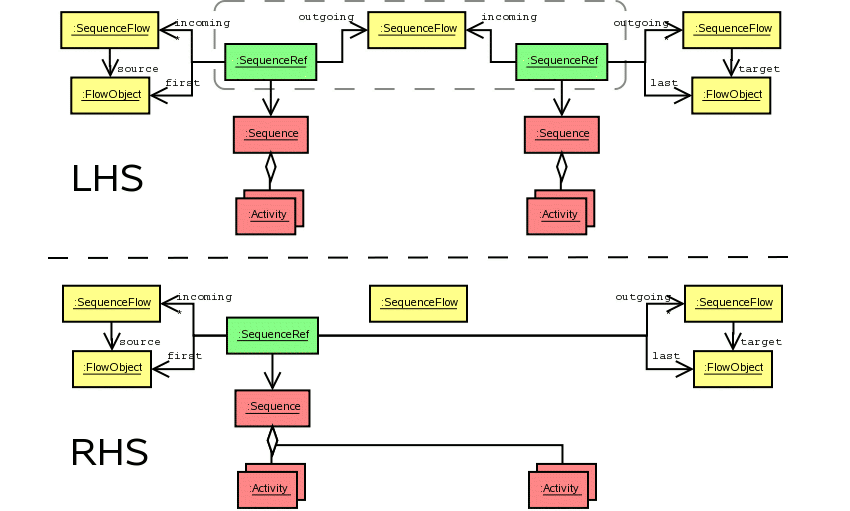
\includegraphics[width=.8\textwidth]{figures/impl/rules/sequenceRule.png}
	\caption[Sequence Rule]{The Sequence Rule}
	\label{fig:seqRule}
\end{figure}

The rule engine will look for occurrences of Sequence Flows being \verb|outgoing| of one and \verb|incoming| of another Sequence Reference. If this is the case the sequences referenced by the Sequence References are merged, preserving the order of the child elements. The first Sequence Reference's \verb|first| and \verb|incoming| elements will be the \verb|first| and \verb|incoming| of the new sequence and the second Sequence Reference's \verb|last| and \verb|outgoing| elements will be the \verb|last| and \verb|outgoing| elements of the new sequence. Finally the second sequence, together with its Sequence Reference, can be removed from the model.

\subsubsection*{Block Rule}
The \emph{Block Rule}, shown in figure \ref{fig:blockRule}, will identify blocks defined by a forking and a merging Gateway and create a new block structure corresponding to the type of the forking Gateway. The type of the merging Gateway can not be taken into account yet. After the block structure has been created all sequences starting at the forking Gateway and ending at the merging Gateway will be put into the block structure. Finally the sequence holding the forking Gateway and the sequence holding the merging Gateway will be combined similar to the \emph{Sequence Rule}, so that the block can then be integrated into a larger sequence.

\begin{figure}[ht]
	\centering
	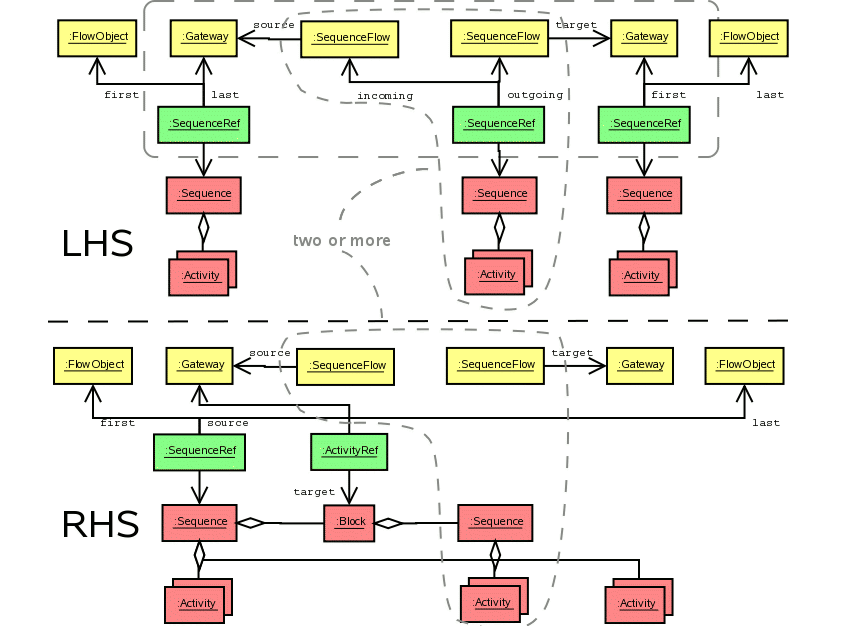
\includegraphics[width=.8\textwidth]{figures/impl/rules/blockRule.png}
	\caption[Block Rule]{The Block Rule}
	\label{fig:blockRule}
\end{figure}

This rule requires that there is more than one sequence in between the Gateways and that there are no sequences starting at the merging Gateway and \emph{not} ending at the forking Gateway and vice versa.

\subsubsection*{Loop Rule}
The \emph{Loop Rule}, shown in figure \ref{fig:loopRule}, is basically very similar to the \emph{Block Rule}. The main difference is that there must not be an arbitrary number of sequences from the first to the second Gateway but exactly one sequence from the first to the second and exactly one sequence from the second to the first. Further, the first Gateway has to have one more incoming Sequence Flow and the second Gateway one more outgoing Sequence Flow, that is, the entry to and the exit from the loop. As shown earlier in figure \ref{fig:normalization_example} after the Normalization stage both \emph{while} and \emph{until} loops will have this form and thus are covered by this rule.

\begin{figure}[ht]
	\centering
	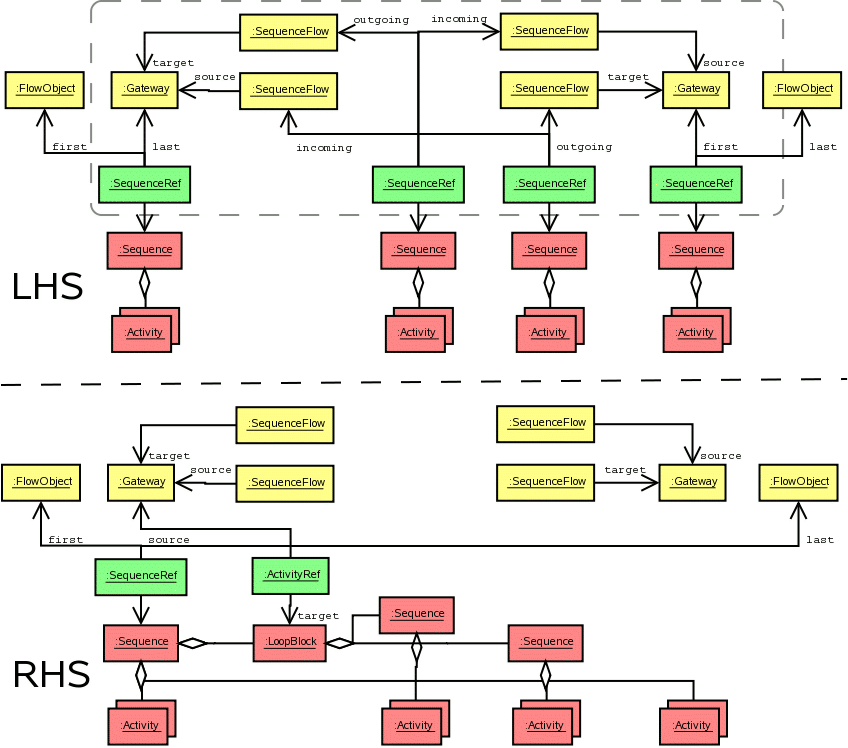
\includegraphics[width=.8\textwidth]{figures/impl/rules/loopRule.png}
	\caption[Loop Rule]{The Loop Rule}
	\label{fig:loopRule}
\end{figure}

When executed, the sequence from the first to the second Gateway (the until-part) will be copied and inserted before the loop structure, since it has to be executed at least once. The sequence from the second Gateway back to the first Gateway (the while part) will be part of the loop's body, together with the copy of the first sequence. The loop condition will be taken from one of the Sequence Flows going out of the second Gateway, depending on which Sequence Flow's condition is a Expression and which is the default.


\subsection{Cleaning Up}

This last stage of the mapping is intended to clean up the target model of redundancies and defects that may have arisen during the mapping.

This list is showing some possible actions for the clean up stage:
\begin{itemize}
	\item remove no-op activities resulting from the Activities inserted in the Normalization stage
	\item resolve unnecessary nesting, for instance sequences nested in sequences
	\item resolve singleton sequences
\end{itemize}

Remember that the Clean Up stage could not be implemented for JIAC IV, since the existing JIAC metamodel is implemented using JAXB which is not compatible with EMT and thus can not be used in its rule patterns.



\section{Open Issues}
\label{sec:mapping_openissues}

Like for the editor there are still some open issues concerning the implementation of the mapping.


\subsection{The Mappings}

Both the mapping to BPEL and to JIAC are not yet fully implemented.
Some of the mappings given in the BPMN Specification are somewhat ambiguous or very difficult to implement, which is why they have been postponed for now.
The mapping to JIAC is not fully specified yet and will need further refinement in some points. Currently the mapping is focused on the planelements, while the mapping to agents is at a very early stage.

Further, the current mapping is addressing JIAC IV, which will be replaced by JIAC TNG soon. The mapping will have to be changed then. Fortunately the metamodel for JIAC TNG will be based on EMF, so it will be easier to integrate in the rule based approach, including a working Clean Up stage.

% 
% \subsection{Custom Artifacts}
% \label{sec:custom_artifacts}
% 
% The Business Process Modeling Notation may be extended by custom \emph{Artifacts}. While the existing elements may not be altered and no additional Flow Objects should be introduced, modelers and modeling tools are free to add non-standard elements as Artifacts, which can be connected to the other elements via Associations. Examples for Artifacts that are currently part of the BPMN are Data Objects, Groups and Text Annotations.
% 
% It might be interesting for the mapping to JIAC to introduce custom Artifacts. These new Artifacts could represent the concepts of ontologies, agents and agent platforms (see figure \ref{fig:bpmn_agents}), which do not have a representation in the original BPMN.
% 
% \begin{figure}[htp]
% 	\centering
% 	\includegraphics[width=.8\textwidth]{figures/impl/bpmn_agents.png}
% 	\caption[Custom Artifacts]{Mockup of custom Artifacts representing agents and agent platforms}
% 	\label{fig:bpmn_agents}
% \end{figure}
% 
% Introducing those artifacts would solve the problems with mapping Pools and Processes to agents: While it might seem reasonable to map Pools to platforms and Lanes to agents this does not harmonize with mapping Processes to plan elements, and even if a Pool is mapped to a single agent this would result in a $1:1$ relation between agents and plan elements, which is not wanted. However, using Artifacts to represent agents and platforms they can be arbitrarily associated to Pools, allowing $n:m$ relations of agents and plan elements.


\subsection{Unstructured Workflows}

% unstructured workflows
The current rules do not yet support the transformation of unstructured workflows. The normalization of unstructured workflows, as described in section \ref{sec:mda_mapUSWF}, will require a number of additional, elaborate rules, but we are confident that even those rules will be possible with the current approach.

% blöcke mit unterschiedlichen splits und joins (deadlock, MI), insb AND-OR, AND-XOR
The existing Block Rule and Loop Rule will have to be completed by taking the joining Gateway into account. Currently the type of the decision structure is determined only by the splitting Gateway: If the split is a AND-Gateway, a parallel structure is created, in the case of a XOR-Gateway an exclusive decision structure is created, and so on.

If the joining gateway is of a different type this can result in deadlocks and loss of synchronization, that is, multiple instances of the same activity being active at the same time. While it may be a good thing that it is not possible to accidentally cause a deadlock, multiple instances can be intended by the modeler. In this case, for instance when a splitting AND-Gateway is followed by a joining OR-Gateway, the remaining workflow after the Gateway would have to be encapsulated in a second process, which can then be called each time the workflow reaches the end of the decision structure.

Another situation, where splitting and joining Gateways of different type are useful, is that of a splitting AND-Gateway and a joining XOR-Gateway: In this case the workflow should be continued right after the first branch has completed, not waiting for the others. This could be achieved by the use of concurrent flow and auxiliary variables.
\\
\\

In this chapter we described how the transformation tool was implemented. We explained the several stages of the mapping and introduced the reader to the most important transformation rules.

The next chapter will give some examples to illustrate the transformation from BPMN to JIAC.